\chapter{Revis\~ao da literatura especializada - Fundamenta\c{c}\~ao te\'orica}
\label{chapter:odometriavisual}
%\setlength{\headheight}{52pt} % ...at least 51.60004pt
%----------------------------------------------------------------------

\textcolor{blue}{Esta seção deve conter a Revisão Bibliográfica da sua proposta de dissertação de acordo com as instruções normativas descritas.}

\section{Odometria Visual}
\label{sec:odometriavisual}

A odometria visual que em inglês significa visual odometry (VO), também conhecida como egomotion, é abordado na área da visão computacional como sendo o processo para  estimar a posição atual (pose) de um agente (por exemplo, veículo, humano e robô) usando apenas a entrada de uma ou várias câmeras anexadas a ele. Domínios de aplicação incluem robótica, computação vestível, realidade aumentada e automotiva \cite{fraundorfer2011visual}. O VO é um caso particular de uma técnica conhecida como Estrutura do Movimento (SFM)  que aborda o problema da reconstrução 3D da estrutura do ambiente e das poses da câmera a partir de conjuntos de imagens sequencialmente ordenados ou não-ordenados \cite{yousif2015overview}.

De acordo com \cite{fraundorfer2011visual}, o termo Visual Odometry (VO) foi cunhado em 2004 por Nister em seu documento de referência \cite{nister2004visual}. O termo foi escolhido por sua semelhança com a odometria das rodas, que estima incrementalmente o movimento de um veículo, integrando o número de voltas de suas rodas ao longo do tempo. Da mesma forma, o VO opera estimando incrementalmente a pose do veículo através do exame das mudanças que o movimento induz nas imagens de seus sensores a bordo. A vantagem do VO em relação à odometria da roda é que o VO não é afetado pelo deslizamento da roda em terrenos irregulares ou outras condições adversas.

Foi demonstrado que, em comparação com a odometria da roda, o VO fornece estimativas de trajetória mais precisas, com erros de posição relativa variando de 0,1 a 2\% \cite{wirth2013visual}, \cite{fraundorfer2011visual} - \cite{nawaf2017towards}. Essa capacidade faz do VO um complemento interessante à odometria das rodas e, adicionalmente, a outros sistemas de navegação, como as Unidades de Medição Inercial (IMUs).

\subsection{Odometria Visual Subaquática}
\label{sec:odometriavisualsubaquatica}

A técnica de VO está se tornando popular nos AUVs para navegação, manutenção de estações e fornecimento de informações de feedback para manipulação.
A saída da odometria visual é frequentemente combinada com as IMUs para fornecer uma alternativa mais barata aos DVLs e sistemas de navegação inercial (INS) \cite{bellavia2017selective}, \cite{wirth2013visual} e \cite{yousif2015overview}. No entanto, as limitações da visão subaquática são amplamente conhecidas e seu desempenho depende de muitos fatores, como visibilidade, iluminação e distorção resultantes de diferentes índices de refração. De acordo com \cite{fraundorfer2011visual}, para que o VO funcione efetivamente, deve haver iluminação suficiente no ambiente e uma cena estática com textura suficiente para permitir a extração de movimentos aparentes. Além disso, os quadros consecutivos devem ser capturados, garantindo que eles tenham sobreposição de cena suficiente.
%% ------------------------------------------------------------------------- %%

\section{Métodos de Odometria Visual}
\label{sec:metodosdeodometriavisual}

Nos últimos anos, muitos métodos de VO foram propostos, que podem ser divididos em métodos de câmera monocular e estéreo \cite{yousif2015overview}. Esses métodos são posteriormente divididos em correspondência de recursos (recursos correspondentes em vários quadros), rastreamento de recursos (recursos correspondentes em quadros adjacentes) e técnicas de fluxo óptico (com base na intensidade de todos os pixels ou regiões específicas nas imagens sequenciais). De acordo com \cite{wirth2013visual}, o pipeline básico do algoritmo de odometria visual consiste nas seguintes etapas (independentemente do tipo de câmera): primeiro, os pontos-chave são identificados em cada quadro da câmera e os descritores de recursos para esses pontos são extraídos. Em seguida, a profundidade de cada ponto de referência é estimada usando estéreo, estrutura de movimento ou uma câmera de profundidade separada. Posteriormente, os recursos são correspondidos nos prazos e a transformação de corpo rígido que melhor alinha os recursos entre os quadros é estimada. O resultado desse processo é uma estimativa do movimento da câmera entre os quadros e, portanto, é necessário integrar esses dados ao longo do tempo para obter a posição e orientação absolutas do veículo. Normalmente, esse resultado final é refinado com uma otimização offline (ou seja, ajuste de pacote), cujo tempo de computação cresce com o número de imagens \cite{fraundorfer2011visual}, \cite{nawaf2017towards}. A Figura~\ref{fig:Figures/dgblocoVO} apresenta uma sequência típica para algoritmos VO de acordo com \cite{yousif2015overview}.
\ \\
\begin{figure}[!htb]
	\centering	
	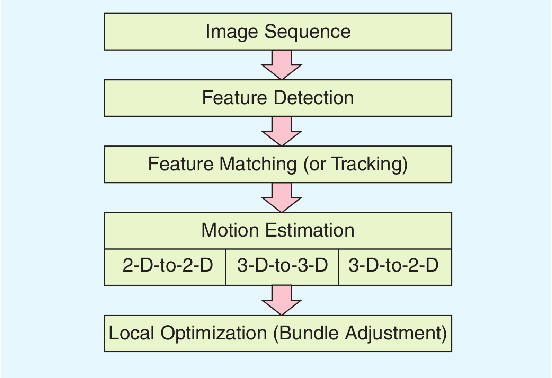
\includegraphics[width=0.5\textwidth]{Figures/DiagramaDeBlocosVO.png}
	\caption{Um diagrama de blocos mostrando os principais componentes de um componente de odometria visual \cite{yousif2015overview}.}
	\label{fig:Figures/dgblocoVO}
\end{figure}
\ \\
%% ------------------------------------------------------------------------- %%

\subsection{Visual Monocular}
\label{sec:visualmonocular}

De acordo com \cite{yousif2015overview}, no VO monocular, os pontos de recurso precisam ser observados em pelo menos três quadros diferentes (observe os recursos no primeiro quadro, re-observe e triangule em pontos 3D no segundo quadro e calcule a transformação no terceiro quadro, Armação). Uma questão importante no VO monocular é o problema de ambiguidade da escala. Ao contrário dos sistemas de visão estéreo em que a transformação (rotação e translação) entre os dois primeiros quadros da câmera pode ser obtida, a transformação entre os dois primeiros quadros consecutivos na visão monocular não é totalmente conhecida (a escala é desconhecida) e geralmente é definida como um valor predefinido . Em \cite{wirth2013visual}, esses problemas também são considerados e descritos. Segundo o autor, sistemas que usam apenas uma câmera precisam de movimento de translação para estimativa de movimento em 3D e todas as medições precisam ser dimensionadas por um fator desconhecido para estar em uma escala métrica.

O uso de uma câmera estéreo calibrada supera os dois problemas mencionados, pois as coordenadas 3D dos pontos correspondentes em um único par de imagens esquerda/direita podem ser calculadas por triangulação.

A Figura~\ref{fig:Figures/MonocularVOSystem} apresenta as poses relativas entre as câmeras que visualizam o mesmo ponto 3D são calculadas combinando os pontos correspondentes na imagem 2D. Se a localização 3D dos pontos for conhecida, pode ser usado um método 3D para 3D ou 3D para 2D. As poses globais são calculadas concatenando as transformações relativas em relação a um quadro de referência (pode ser definido como o quadro inicial) \cite{yousif2015overview}
\ \\
\begin{figure}[!htb]
	\centering	
	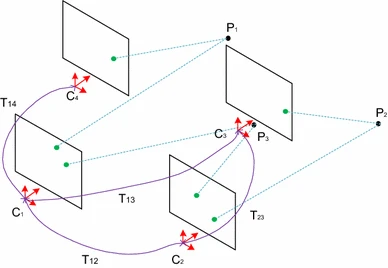
\includegraphics[width=0.6\textwidth]{Figures/MonocularVOSystem.png}
	\caption{Um exemplo de sistema VO monocular.}
	\label{fig:Figures/MonocularVOSystem}
\end{figure}
\ \\
As abordagens de VO foram apresentadas também para o domínio subaquático. Usando pipelines que incluem rastreamento de recursos e estimativa de movimento, esses sistemas são capazes de calcular transformações planares \cite{huang2017visual} ou seis graus de liberdade (DoF) \cite{wirth2013visual}, \cite{corke2007experiments} incrementais da pose da câmera. Medidas inerciais também podem ser incluídas para melhorar o desempenho \cite{creuze2017monocular}.

De acordo com \cite{bellavia2017selective}, os ambientes subaquáticos são tipicamente caracterizados por imagens não estruturadas, ruidosas e altamente texturizadas, com padrões repetitivos e más condições de iluminação local (efeitos de vinheta e outros artefatos). Consequentemente, os pontos-chave da imagem são difíceis de rastrear e corresponder corretamente debaixo d'água, mesmo se forem empregados detectores/descritores de recursos estáveis e robustos, como a transformação de recurso invariante em escala (SIFT) \cite{lowe2004distinctive}, os recursos robustos acelerados (SURF) \cite{bay2006surf} ou descritores de recursos com base nos momentos de Zernike \cite{eustice2008visually}, \cite{kim2009pose}.

A maioria das soluções subaquáticas propostas prefere configurações estéreo em vez de monoculares para melhorar a robustez e a precisão da saída, evitando problemas como os citados antes \cite{bellavia2017selective}, \cite{kim2013real}.
%% ------------------------------------------------------------------------- %%

\subsection{Visual Estéreo}
\label{sec:visualestereo}
\ \\
Usando o mesmo conceito do sistema visual humano, o sistema de visão estereoscópica ou estereoscópica emprega um conjunto de câmeras binoculares, como mostrado na Figura~\ref{fig:Figures/ImagensSimutaneas}. Segundo os autores em \cite{stivanello2008correspondencia}, um sistema estéreo pode extrair informações da cena observada recuperando dados de profundidade de um ponto no espaço a partir da distância relativa entre dois pontos. Essa diferença nas coordenadas dos pontos correspondentes às projeções é chamada disparidade.
\ \\
\begin{figure}[!htb]
	\centering	
	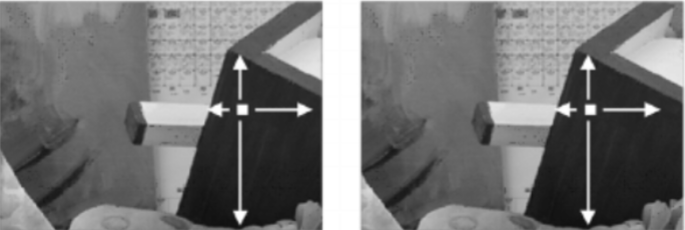
\includegraphics[width=0.7\textwidth]{Figures/ImagensSimutaneas.png}
	\caption{Imagem de duas lentes simultâneas \cite{stivanello2008correspondencia}.}
	\label{fig:Figures/ImagensSimutaneas}
\end{figure}
\ \\
A geometria necessária para fornecer a terceira dimensão é baseada no conceito de geometria epipolar, onde duas câmeras são apontadas para a mesma cena em duas posições distintas, resultando em várias conexões geométricas entre elas e, portanto, fornecendo os pontos 3D, epipolar. A geometria é apresentada com mais detalhes em \cite{bappy2012study}.

\begin{figure}[!htb]
	\centering	
	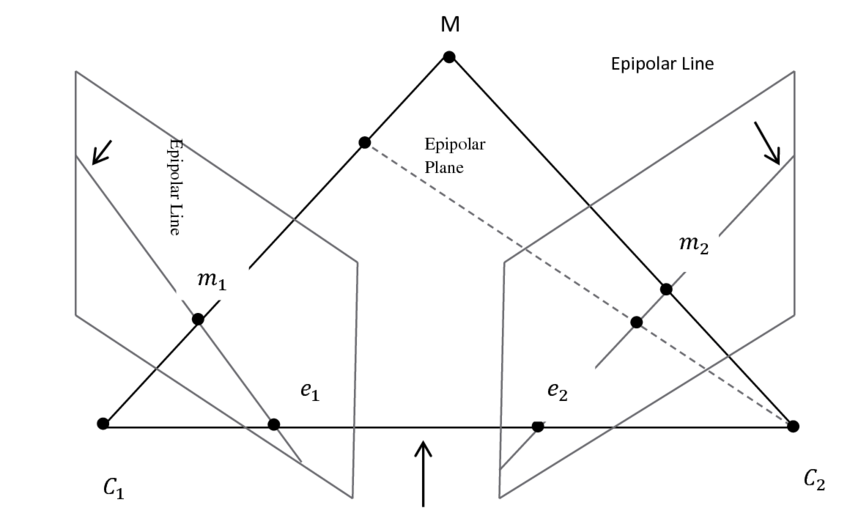
\includegraphics[width=0.5\textwidth]{Figures/EpipolarGeometry.png}
	\caption{Conceito de geometria epipolar \cite{bappy2012study}.}
	\label{fig:Figures/EpipolarGeometry}
\end{figure}
\ \\
A odometria visual (VO) é o processo de estimar o movimento de um veículo em movimento usando a entrada de vídeo de suas câmeras a bordo.

No VO estéreo, o movimento é estimado pela observação de recursos em dois quadros sucessivos (nas imagens direita e esquerda). Na Figura~\ref{fig:Figures/Clound3DPoints}, são mostrados quadros rastreados para formar uma nuvem de pontos 3D esparsos do ambiente e podem ser usados como base para a localização.
\ \\
\begin{figure}[!htb]
	\centering	
	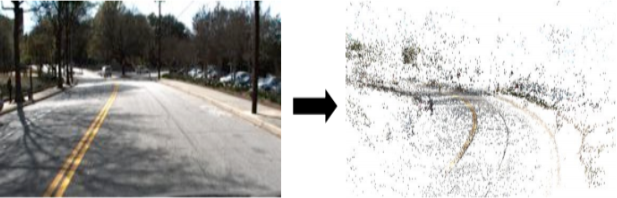
\includegraphics[width=0.8\textwidth]{Figures/Clound3DPoints.png}
	\caption{Os quadros rastreados formam uma nuvem de pontos 3D \cite{stivanello2008correspondencia}.}
	\label{fig:Figures/Clound3DPoints}
\end{figure}
\ \\
De acordo com os autores em \cite{stivanello2008correspondencia}, uma das principais vantagens da visão estéreo é que as imagens armazenam uma quantidade enorme de informações significativas, mesmo sem a necessidade de mover a câmera, além disso, fornecem alta precisão da localização, provando ser barata. solução em comparação com outros sensores de proximidade. Em \cite{zhou2017robust}, devido à certa linha de base entre as câmeras esquerda e direita, o problema de escala de ambiguidade é estabelecido e provado que não existe no VO estéreo. Além disso, o VO estéreo pode estimar o 6-Degree of Freedom (DOF) e o sensor do movimento do ego, o que não diz respeito ao tipo de ambiente em que o sistema trabalha. Atualmente, existem dois tipos de métodos de VO estéreo, 3D-3D e 3D-2D.

De acordo com \cite{yousif2015overview}, essa estimativa de movimento 3D-3D é realizada triangulando pontos de recurso 3D observados em uma sequência de imagens. A transformação entre os quadros da câmera é então estimada minimizando a distância euclidiana 3D entre os pontos 3D correspondentes.

Os autores também discutiram sobre o método de estimativa de movimento 3D-2D semelhante à abordagem anterior, mas aqui o erro de re-projeção 2D é minimizado para encontrar a transformação necessária. Novamente, o número mínimo de pontos requeridos varia com base no número de restrições no sistema.
Embora esses métodos de VO estéreo tenham se mostrado promissores, existem alguns problemas em relação à captura de imagens, gerando desvio de trajetória e valores discrepantes, como condições de iluminação, textura ao redor, presença de água, neve, desfoque de movimento, presença de sombras, semelhança visual, configuração degenerada e oclusões.

Com o objetivo de avaliar a melhor abordagem para estimativa de localização, a comparação de desempenho entre as abordagens de VO estéreo e VO monocular foi realizada em \cite{chen2015performance}. Figura~\ref{fig:Figures/DemoPerMonocular}, a trajetória no movimento de curvatura pode ser facilmente distinguida com o caminho de referência no modo monocular. O valor da distância percorrida é de 6,3\%, o principal motivo é que o resultado da correspondência monocular não é robusto o suficiente para fornecer uma boa estimativa de movimento quando o veículo está sob a dinâmica de viragem. Além disso, há um problema de ambiguidade de escala no resultado.

Portanto, o sistema VO estéreo tem desempenho mais estável que o sistema monocular, e a superioridade pode ser verificada através do experimento de tornar dinâmico em \cite{chen2015performance}.

Figura~\ref{fig:Figures/AnaliseOdometria}, é mostrada a comparação de desempenho entre o sistema de integração INS (Sistema de Navegação Inercial)/GNSS (Sistema Global de Navegação por Satélite), que é um dos mais usados na área de navegação, e a abordagem VO (Odometria Visual), respectivamente para sistemas monocular e estéreo. A taxa de amostragem mais alta tem melhor desempenho tanto na trajetória pura quanto na TD (Distância percorrida), tanto E (leste) (m) quanto N (norte) (m), quando o veículo passa por algumas áreas onde a qualidade do sinal GPS recebido é instável, o INS/GPS MEMS (Micro Sistemas Eletromecânicos) com o esquema fracamente acoplado gerará facilmente piores soluções de navegação \cite{chen2015performance}.
\ \\
\begin{figure}[!htb]
	\centering	
	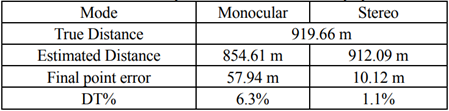
\includegraphics[width=0.6\textwidth]{Figures/AnaliseOdometria.png}
	\caption{A análise numérica de dois sistemas de odometria visual em que a comparação é curva é mostrada na Figura~\ref{fig:Figures/DemoPerMonocular} e na Figura~\ref{fig:Figures/DemoPerEstereo}
	\cite{chen2015performance}.}
	\label{fig:Figures/AnaliseOdometria}
\end{figure}
\ \\
\begin{figure}[!htb]
	\centering	
	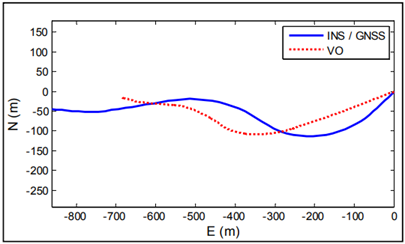
\includegraphics[width=0.6\textwidth]{Figures/DemoPerMonocular.png}
	\caption{Demonstração de VO monocular de desempenhos com mais distorção
	\cite{chen2015performance}.}
	\label{fig:Figures/DemoPerMonocular}
\end{figure}
\ \\
\begin{figure}[!htb]
	\centering	
	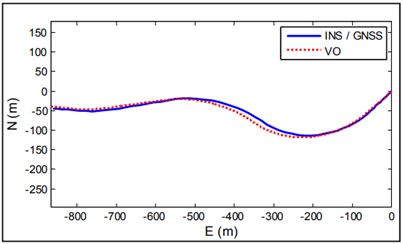
\includegraphics[width=0.6\textwidth]{Figures/DemoPerEstereo.png}
	\caption{VO estéreo, demonstrativa de desempenho mais estável \cite{chen2015performance}.}
	\label{fig:Figures/DemoPerEstereo}
\end{figure}
\ \\
%% ------------------------------------------------------------------------- %%

\section{Visual SLAM}
\label{sec:visualslam}

De acordo com \cite{yousif2015overview}, \cite{fraundorfer2011visual} SLAM é uma maneira de um robô se localizar em um ambiente desconhecido, enquanto constrói incrementalmente um mapa de seus arredores. O SLAM foi extensivamente estudado nas últimas décadas, resultando em muitas soluções diferentes usando sensores diferentes, incluindo sensores de sonar, sensores de infravermelho e scanners LASER. Recentemente, houve um interesse crescente no SLAM baseado em visual, também conhecido como V-SLAM, devido às informações visuais ricas disponíveis nos sensores de vídeo passivos de baixo custo em comparação aos scanners LASER.

De acordo com \cite{fraundorfer2011visual}, \cite{nister2004visual}, o objetivo do V-SLAM é obter uma estimativa global e consistente do caminho do robô. Isso implica manter um controle de um mapa do ambiente (mesmo no caso em que o mapa não é necessário per se) porque é necessário perceber quando o robô retorna a uma área visitada anteriormente, esse processo é conhecido como detecção de fechamento de loop. Quando um fechamento de loop é detectado, essas informações são usadas para reduzir a deriva no mapa e no caminho da câmera. De acordo com \cite{wirth2013visual}, os algoritmos para odometria visual - em oposição aos algoritmos SLAM completos - concentram-se em estimativas rápidas de movimento quadro a quadro, sem manter um grande histórico de fechamento de loop.

A ênfase está em medições precisas em altas frequências. Entender quando ocorre um fechamento de loop e integrar eficientemente essa nova restrição no mapa atual são dois dos principais problemas do V-SLAM. Uma das principais desvantagens da implementação das técnicas do V-SLAM depende do tempo de computação e utiliza recursos que, por sua vez, crescem significativamente para grandes ambientes \cite{nawaf2017towards}. Em \cite{strasdat2012visual} é apresentada uma pesquisa extensa considerando outros aspectos relacionados ao V-SLAM e aplicações similares.
%% ------------------------------------------------------------------------- %%

